\section{Software Design}
  Following the design of the mechanical and electrical aspects of the rover was that of the software as hosted by the RCE as well as for user control and interaction. The section covers the design process undertaken before and during the development of the software for all aspects of the project. The software design and development processes were highly iterative as many of the design choices had to be made after realisation of the technology capabilities and conversely, many of the technology choices were made based on what was required on a more functional and detailed level at design time. The two processes are separated as far as possible in this report for a friendlier structure, however, much of the design detail is included in the development sections.
  
  The design stage initiated with an overview of the requirements, a plan of the designed structures of each of the subsystems as categorised in the overview and descriptions of the technologies that were chosen for development.
  
  \subsection{Systems Overview in Context}
    An attempt was made to mimic the communications and software structures and patterns used for MSL (and other similar missions) and as such, the software system for this project resembles the three component structure consisting of a system on the rover, the software employed for the collection of relay satellites and ground-based DSN hardware, and the client front-end software as used by the MSL team. Figure~\ref{fig:specs-functionalBreakdown} already highlights the basic breakdown of the software systems. As discussed in Section~\ref{subsubsec:rover-equivalence}, the three major software subsystems by name included the Rover Compute Element (RCE) and the Robot Sequencing and Visualisation Program (RSVP) divided further into the Server and the Client.
    
    The RCE was hosted by the computational hardware on the rover (the Intel Edison board, here-onwards referred to as the RCE board) and required control of hardware, sensory and digital input and communication with the RSVP Server in order to fulfil the end requirements. This imposed the need upon the RCE to be able to read from and control the hardware inputs and outputs on the RCE board. For communication, the RCE was to make use of the on-chip WiFi module to send and receive data which would make up the commands, telemetry and video stream.
    
    The RSVP Server was a standalone server process serving as the middle-man between the RSVP Client and the RCE with respect to telemetry, control and video data. The Server established connections with the RCE for data message and video stream type communications and was required to act as a broadcast node to allow for multiple RSVP Client instances to receive the data messages and the video stream. Details on the network topologies, specifically those of the video broadcasting component, are discussed in the structure plans to follow. The RSVP server also hosted the RSVP Client web application to be served and coordinated control access by the active clients.
    
    The RSVP Client as served by the RSVP Server was a web application which was required to facilitate user input for control of the rover, display the video feed from the RCE as broadcast by the Server as well as provide telemetry received via data messages. As described further in the following design sections, the RSVP Client consisted of a front-end component visible in the browser or any web-view as well as an underlying system managing the flow of data through the application and handling the communication between it and the RSVP Server. State and user input data was to be sent to and received by the Server and the video data received to be displayed in the video element within the interface.

    \begin{figure}[h!]
      \centering
      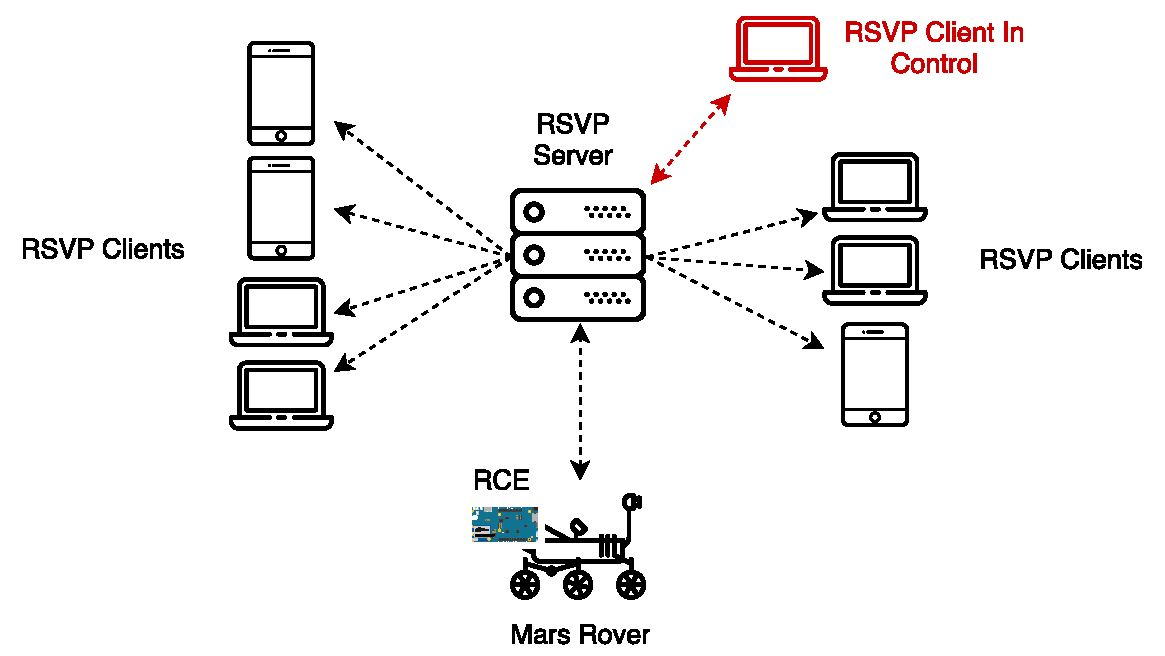
\includegraphics[width=0.7\linewidth]{figures/softDesign-useOverview}
      \caption[Diagramatic depiction of a typical use scenario of the software system]{Diagramatic depiction of a typical use scenario of the software system}
      \label{fig:softDesign-useOverview}
    \end{figure}

    An overview of the entire software system on a very high level is shown in Figure~\ref{fig:softDesign-useOverview}, a typical scenario involving the operational rover, the RSVP server in communication with the RCE and multiple RSVP Clients connected to the Server. The intention was to have the system be capable of allowing multiple devices on the network to connect to and interact with the system and one of the devices to have rover control access. The RSVP Server would manage the connected Clients and decide which of them would be able to control the rover. The principle behind the choice of which Client becomes the controlling Client is discussed later on.
    
  \subsection{Plan of Structure}
    In order to effectively coordinate the design and development of the software system as a whole, structural plans of the system and the subsystems within were constructed. The plans also aided the realisation of requirements and, further, choices of software technologies to use for each of the subsystems and components. The high level structure of the three subsystems and their interconnectedness was designed before constructing more detailed perspectives of each of them.
    
    \subsubsection{System Architectural Structure}            
      Figure~\ref{fig:softDesign-sysArchitectureStructure} is a high-level diagram showing a single-client scenario involving the three primary software subsystems and the means by which they were to communicate and interact. The solid arrows indicate wired connections and these exist on the RCE board for, as on the left, hardware communication and interfacing with sensory devices such as the camera. The RCE uses the wireless module to transmit video data and message data to the Server via the wireless module on the RCE board. The RSVP Server then offers the application source for the RSVP Client to be requested and loaded. Control, telemetry and video data is then sent and received between the RSVP Client and Server.

      \begin{figure}[h!]
        \centering
        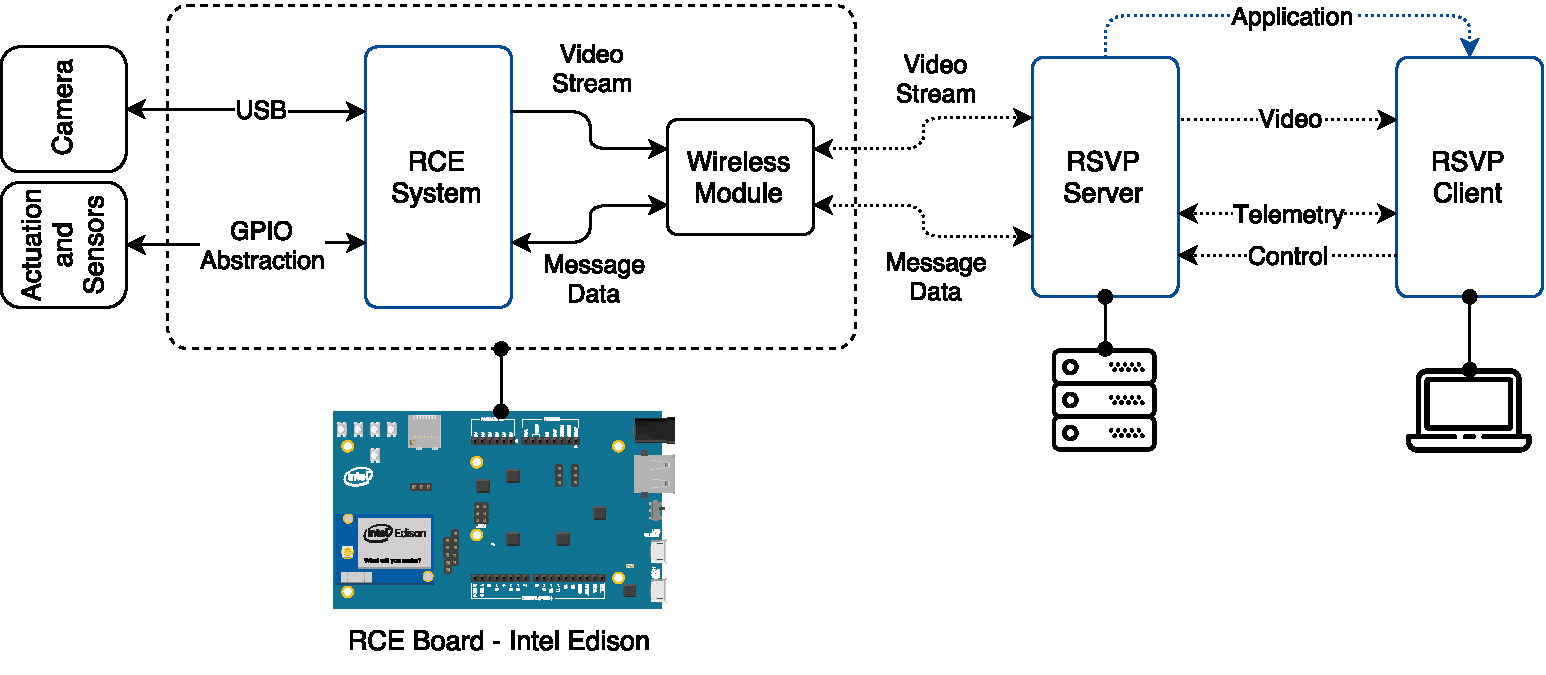
\includegraphics[width=1\linewidth]{figures/softDesign-sysArchitectureStructure}
        \caption[Diagram outlining the basic software system component structure]{Diagram outlining the basic software system component structure}
        \label{fig:softDesign-sysArchitectureStructure}
      \end{figure}
      
      As mentioned previously, the RSVP Server's primary role was to relay data between the RSVP Client and the RCE. Employing this structure for the flow of data allowed for many RSVP Client instances to exist and interface with the system. Not shown in Figure~\ref{fig:softDesign-sysArchitectureStructure} is the case where there are $N$ RSVP Clients on the network whereby one client would be in control of the rover, using the control, telemetry and video communication channels, and $N-1$ Clients would be receiving telemetry and video data only. Throughout the software design process, as much of the computational burden anticipated to exist in the system was offloaded onto the RSVP Server simply due to the fact that the RCE had the most severe computational performance limitations. The RSVP Server could be scaled to provide any required performance and thus could absorb functional components that were computationally taxing, an example of which is handling a large number of client connections that all require video and telemetry data. Communication specifics between all of the subsystems in Figure~\ref{fig:softDesign-sysArchitectureStructure} will be discussed in the design sections that follow as well as in the development sections.
      
      It can be seen in Figure~\ref{fig:softDesign-sysArchitectureStructure} that data transmission between all components of the system are grouped into two main channels: video data and message data. The separation of the two is made clearer in Section~\ref{subsubsec:rsvpServersPlan} which discusses the broadcast topology intended for use for the video data and how the data and the characteristics of the required communication naturally differ from that of telemetry and control data. Splitting of the two flows of data also allowed for finer control over the transmission in terms of setup sequences and during operation. As such, the message data channel between the Server and a Client was split on the basis of function.
      
  \subsection{Technology Choices}
    \subsubsection{Common Platform Flavour}
      The fact that the RCE board's computer supported the use of Linux as an operating system presented an opportunity to have all aspects of the software system follow suit in this regard, specifically the RSVP Server. The Server was intended to be flexible in form-factor to facilitate the open-sourcing secondary objective of the project and for the purpose of the system developed for this report, it was chosen to be a PC capable of running a distribution of Linux. Most distributions of Linux offer the stability and performance required by server-type processes and applications which explains the popularity of the operating system in network and internet service industries \cite{w3techs_Oct2016} and hence the decision to employ such as the operating system for the Server. The choice between heterogeneous and homogeneous architectures for the software system resolved to a trade-off between the advantage of technological flexibility as in the heterogeneous case and development simplicity in the other. Technological flexibility would have benefited the design in allowing choice of technologies that would better suit each of the subject components, perhaps to optimise resource consumption (storage, computation or even power) or improve compatibility with associated hardware and other components. Due to the limited time-frame of the project as well as there being no specification related to such optimisations, the benefit of the ease of learning and design brought by a homogeneous system weighed in greater than flexibility, together with the abundance of packages and tools available for a Linux-based platform. Using Linux also supported the free, open-source software ideology making it more readily available to those who intend to be involved.
      
      \subheading{JavaScript}\\\\
        With both the RCE and RSVP Server being based on a Linux platform as well as the RSVP Client being web-based (discussed further in Section~\ref{subsubsec:applicationFrontend}), another opportunity to employ a common technology across the system was presented, specifically the use of the JavaScript language most commonly associated with websites and web applications. Using JavaScript across the stack (including the RCE) followed the architecture pattern of homogeneity, simplified the learning process before and during development of the subsystems and minimised anticipated development overhead in terms of software development environments and build tools. Using JavaScript kept the project on a modern, popular and cutting-edge trajectory, a choice backed by it being a widely recognised full-stack solution used for services such as Netflix, Paypal, Medium, Uber, Twitter and Airbnb \cite{nodeusers_2016} \cite{driesbuytaert_2016}. JavaScript's place in an embedded context was found to be increasingly fitting, especially in scenarios where an internet-connected stack could benefit from the seamlessness of technologies as a result. Given that the Intel Edison was a device which comfortably bridged between a embedded environment dedicated to hardware alone and a connected computer with no direct hardware-interface relevance at all, JavaScript provided a good balance between the two areas of software and kept available interoperability with software and tools that could cover the extremes if required. Other benefits include the use of JSON as a well recognised data format, untyped syntax and the semantic depth provided by the object-oriented nature of the language.
        
        JavaScript itself was not the platform choice in entirety and due to the fact that it is an interpreted language, the project required a choice of runtime environment that would be able to be used on both the RCE and the RSVP server. It was found that the most popular server-side runtime for JavaScript projects was Node.js, an asynchronous, event driven, single thread environment that utilises the V8 JavaScript Engine. It was identified that the structure of the stack of this project resembled a typical IoT stack (involving a front-end, back-end and connected devices) and Node.js was the most popular environment for applications that required real-time data synchronisation and connectivity between devices with a growth in usage unlike any other JavaScript runtime or framework \cite{nodejsSurvey_2016}.
        
        \begin{figure}[h!]
          \centering
          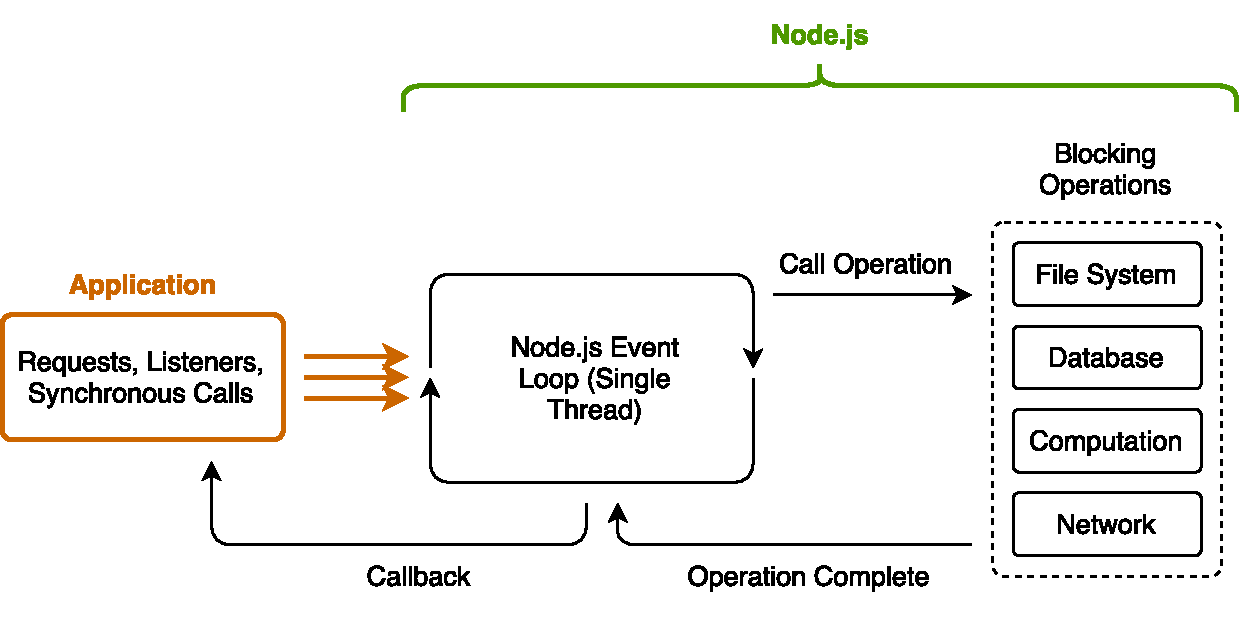
\includegraphics[width=0.9\linewidth]{figures/softDesign-nodeEventLoop}
          \caption[Diagram showing the Node.js architecture's event-loop execution design]{Diagram showing the Node.js architecture's event-loop execution design (adapted from \cite{fig:softDesign-nodeEventLoop_cite1} and \cite{fig:softDesign-nodeEventLoop_cite2})}
          \label{fig:softDesign-nodeEventLoop}
        \end{figure}
        
        A key advantage of the way in which Node.js runs is in the event loop architecture that it utilises, as demonstrated in Figure~\ref{fig:softDesign-nodeEventLoop}. Since Node.js is single threaded, in order to bring asynchronism to an application, at least one point of the software architecture should be sequential in execution, taken care of in the Node.js case with its event loop. The significance of this method of execution is in the advantages that it brings when dealing with operations that block the execution flow. In the context of server applications where requests are fully asynchronous, any operation that blocks handling of such requests will result in poor response performance and a poor end user experience. System operations are normally always blocking in operation and thus Node.js utilises a system library \mintinline{js}{libuv} to offload the blocking calls to system threads, the important point here being that the event loop need not wait for the operation to complete. This means that the left hand side of the flow of execution in Figure~\ref{fig:softDesign-nodeEventLoop} (application requests) is scalable with minimised performance cost, allowing many end users to be connected to and request data from the server at any given time.
        
        Node.js brought with it open-source resources, tools and software modules which greatly improved the development time and opened up what was possible from the perspective of both the RCE and the RSVP Server (and Client, but to a lesser extent). Many of the open-source projects used throughout the software system were chosen during development based on demand and are mentioned in-text in the design and development sections as well as at the end of this report. % TODO: List the open source dependencies
        
        A project worthy of mentioning at this point is one that was in development at the time of writing by NASA, namely Open MCT\footnote{Open MCT: \url{https://nasa.github.io/openmct/}}, a web-based mission control framework utilising Node.js as the server runtime (although the architecture design was intended to be server-agnostic). Open MCT was a great example of how an across-the-stack JavaScript implementation is well suited to a data and communication critical application. Another example of Node.js's place in the aerospace industry was the use of it by United Technologies Corporation Aerospace Systems (UTCAS) to develop a data management system for the lifecycle of EVA spacesuits, a response to a problem identified in the analysis of data which was before hosted across separate and legacy databases \cite{nodejsSpaceSuit_2016}.        
        
      \subheading{ECMAScript 6}\\\\
        Released on the 6th of June 2015, the Sixth Edition of JavaScript, also known as ECMAScript 6 (ES6), introduced a significant range of new features to the language many of which are syntactically unique. It was decided that the project make use of the new edition in order to remain in-sync with modern modules and technologies at the time. In fact, a few features from the Seventh Edition (ES7, released on the 7th of June 2016) were included as well, both additions to the original ES5 and ES5.1 resulting in an added complexity in the build process. The changes to the build process are dealt with in the development section.
        
    \subsubsection{Embedded Software Platform}
      The RCE board's Intel Edison computer ran a default operating system: a custom version of Linux from the Yocto Linux Project maintained and compiled by Intel. The open-source Yocto Project provides the tools and resources to build Linux distributions specifically for embedded targets. Intel's distribution was a modified version of ``Yocto Poky'' and could be flashed onto the Intel Edison using the tools provided. After little experimentation with the distribution, it was found that many of the niceties of a Debian-based operating system were not present, the main issue being the lack of the package manager (\mintinline{js}{apt-get}) and its associated online repositories which would aid the development process. For this reason, a different distribution was chosen for the RCE, ``Ubilinux'', a customised version of ``Debian Wheezy'' which was maintained by Emutex. It was decided that due to mid-project termination of support for Ubilinux from Emutex, Ubilinux would remain the distribution used during development of the rover after which it would be replaced with the latest version of Yocto Poky if time permitted. This would provide an opportunity to build into the distribution the tools confirmed as being required for the operation of the RCE.
    
      Since it is primarily a server runtime, Node.js itself did not have native support for embedded hardware control such as that required for the RCE. It was important to first understand how the hardware was interfaced with from the perspective of the Linux user space\footnote{Linux user space: memory area and separation of execution reserved for application code and some hardware drivers, which sits separate from the kernel space reserved for low level code and drivers} on the Intel Edison. One of the base-level principles around which Linux was developed is the concept of the hierarchical file-system. Most importantly, the file-system need not necessarily consist of files that represent viewable and editable data in the user-owned sense (documents, pictures and other media, for example) but also files that hold system data which have been allowed to propagate from the kernel space to the user space. The system files may represent various hardware components and subsystems, holding state information and allowing control of the hardware through editing of the associated files. The significance of this concept is that the Intel Edison exposes hardware pin access using a virtual file system from the kernel upwards into the user space using \mintinline{js}{sysfs}. When the \mintinline{js}{sysfs} file system is mounted, files organised and structured to represent the GPIOs and other hardware peripherals appear in the user space file hierarchy and if the user has the required permissions, it can read from and write to the files from software. A diagram showing the components of this type of hardware interface on the Intel Edison is shown in Figure~\ref{fig:softDesign-sysfsExample}.
      
      \begin{figure}[h!]
        \centering
        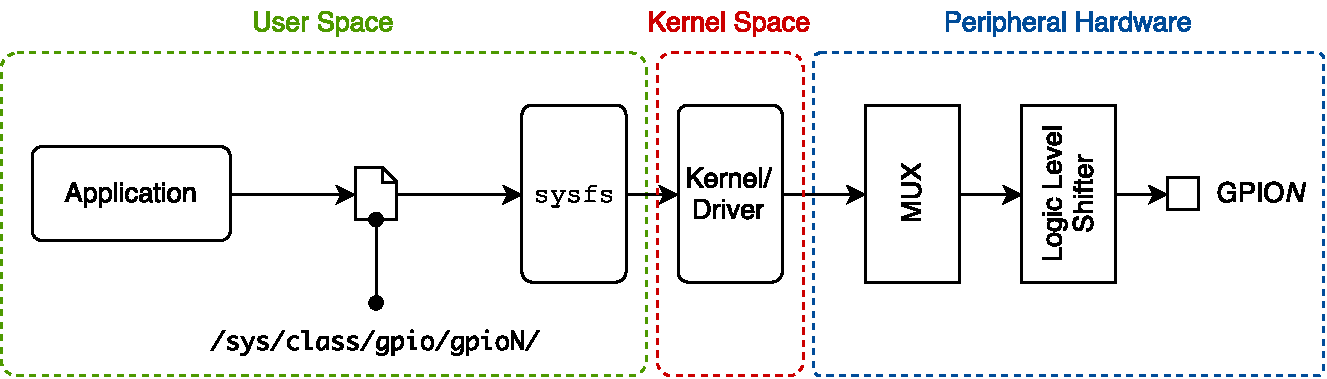
\includegraphics[width=0.8\linewidth]{figures/softDesign-sysfsExample}
        \caption[Simplified diagram showing the interface between peripheral hardware and code running in the Linux user space]{Simplified diagram showing the interface between peripheral hardware and code running in the Linux user space (adapted from \cite{fig:softDesign-sysfsExample_cite1} and \cite{fig:softDesign-sysfsExample_cite2})}
        \label{fig:softDesign-sysfsExample}
      \end{figure}
      
      Atop this method of hardware interface was another abstraction that was available: a C/C++ library, called \mintinline{js}{mraa}, which provided common \mintinline{js}{sysfs} file operations in code allowing for better semantics amongst the large amount of multiplexing required on the Intel Edison board. \mintinline{js}{mraa} also provided JavaScript bindings so that the library could be easily utilised in the RCE software subsystem running in the Node.js environment. This was not the end of the stack, however, as multiple Node.js modules were available that resided atop the JavaScript abstraction of \mintinline{js}{mraa}. Up until this point, little variation in the platform layers was available and this final choice of module formed the primary design choice for the RCE platform. Two robotics framework modules were chosen as candidates based on popularity and compatibility with the Intel Edison (and the Arduino Breakout Expansion), namely ``Johnny-five'' and ``Cylon.js''. Both modules leveraged the object-oriented nature of JavaScript to provide easy interface with the hardware on the RCE board as well as provide the ability to remotely program and command the device on the same network. The architectures of each of the modules were compared and it was found that Cylon.js emphasised the remote scripted topology compared to code that would run local to the device to be controlled. The intention was to have the RCE be independent in operation from any other device (i.e. not be strictly reliant on another device to be online) much like the autonomy of \textit{Curiosity} and therefore Johnny-five (hereafter referred to as J5) was chosen as the framework to use. An example snippet of how one would use J5 is shown in Snippet~\ref{code:softDesign-j5ExampleLed}.
      
      \begin{code}
        \begin{minted}{js}
          import * as five from 'johnny-five',
          
          // Create the board instance
          board = new five.Board();
          
          // Setup listener to wait for board to become ready
          board.on('ready', () => {
            // Create an Led on pin 13
            var led = new five.Led(13);
          
            // Strobe the pin on/off, defaults to 100ms phases
            led.strobe();
          });
        \end{minted}
        \caption{Example initialisation of a device and an LED in J5}
        \label{code:softDesign-j5ExampleLed}
      \end{code}
      
      \begin{figure}[h!]
        \centering
        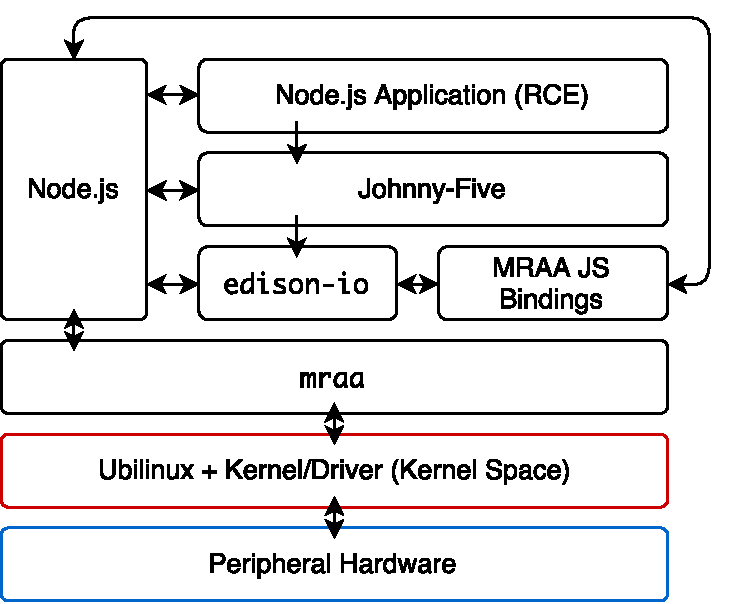
\includegraphics[width=0.5\linewidth]{figures/softDesign-rceHardwarePlatformStack}
        \caption[Diagram of the hardware stack designed for the RCE]{Diagram of the hardware stack designed for the RCE}
        \label{fig:softDesign-rceHardwarePlatformStack}
      \end{figure}
      
      The resulting RCE hardware stack is shown in Figure~\ref{fig:softDesign-rceHardwarePlatformStack} which allowed hardware exposure to the RCE software for all the specified requirements, except the camera, which was handled in a lower-level manner discussed in the development section. A further addition to the stack, \mintinline{js}{edison-io}, is shown in the diagram, which is responsible for dealing with hardware platform specifics in an attempt to keep Johnny-Five and its class and driver implementations as consistent and standard as possible. The \mintinline{js}{edison-io} project is a direct wrapper of \mintinline{js}{galileo-io}, a board support module compatible with the Intel Edison.
      
    \subsubsection{The Web as an Application Front-end}
    \label{subsubsec:applicationFrontend}
      Up until this point, the RSVP Client has been said to be a web application without proper reasoning. The decision was made at the start of the project not without consideration of other front-end platforms. Whilst not explicitly stated in the project specifications, the intention behind the RSVP Client was for it to be a highly accessible application that need not be restricted to within the exhibition space. This follows the theme of the project being targeted at educational environments and general outreach where an application that can be accessed from multiple different devices in multiple locations would prove to be a valuable feature.
      
      The two main categories exist with respect to base-level technologies for the front-end, native applications and web applications, where native refers to applications that are dedicated to the subject device or platform. Investigations made into the popularity of the two application types \cite{jeffSmith_2016}\cite{samShabaan_2016} suggested that at the time of decision, native applications were more commonly used but most likely for specific and repeated tasks or where CPU-intensive computations are required. What was also found, albeit a trivial point, was that the development time, complexity of projects and increased maintenance and skills is required for applications that are to be natively developed but also available across many different types of devices. The web, however, could be considered a universal platform which attempts to bring platform-agnosticism to web content through browsers. The browser can be seen as a technological buffer between the page content and the hardware on which the browser is running.
      
      The project aimed to have the RSVP Client be an application that could be run on as many devices as possible, varying in operating systems, form factors and screen sizes. This objective coupled with the very short development time-frame gave the decision to make the Client a web-based application satisfactory justification. It was also deemed reasonable to make use of the already existing requirement for network-based data communications for the application itself.
      
    \subsubsection{Front-end Framework}
      The RSVP Client could have been developed from first principles or by making use of an already developed front-end JavaScript web-application framework, of which there were an abundance. Many of the frameworks available were created with both user-interface (UI) components and application mechanics in mind. For brevity, a comparison of the candidate frameworks is not shown, however the ones that were considered include AngularJS\footnote{AngularJS: a framework which allows the extension of plain HTML with in-browser JavaScript dependency injection - \url{https://github.com/angular/angular.js}}, ReactJS\footnote{ReactJS: a Facebook developed declarative JavaScript library with a distinct DOM creation and management flow - \url{https://github.com/facebook/react}} and Polymer\footnote{Polymer: a Google developed library come ecosystem which allows the creation of reusable HTML elements with style and functional encapsulation with emphasis on making close use of web standards - \url{https://github.com/Polymer/polymer}}. The chosen framework was Polymer for the following reasons:
      \begin{itemize}
        \item \textbf{Web-components:} Polymer makes heavy use of a particular area of the modern day web standard, the features relating to web components. Web-components allow the encapsulation of functions, features and UI artefacts to result in a component that is re-usable and maintenance-sane. This allows the developer to bring semantic structure to the application in a way which promotes understanding for people who wish to contribute to the project, for example.
        \item \textbf{Shadow-DOM:} Included in the principle of web-components is the Shadow-DOM feature, a mechanism of HTML encapsulation which includes style and associated methods and properties.
        \item \textbf{Declarative Data:} Polymer comes with a rich data management mechanism allowing for the declarative construction of data flow through the application, an area of application design that can get complex and difficult to scale.
        \item \textbf{Polymer Elements Catalog:} Google have provided a large catalog of ready-made Polymer elements which are commonly required UI and application components for easy development. In addition to the Polymer Catalog are elements that have been developed by third parties and made available for use in an open-source manner.
      \end{itemize}
      
      The Polymer Project had also made indications towards making the framework ES6 compliant meaning the framework would remain a sustainable choice for the RSVP Client application.
      
    \subsubsection{Message Data Communication}
      Message data communication was required between the RCE and RSVP Server as well as between the RSVP Server and the RSVP Client. This data would be a structured payload which in JavaScript amounts to a JSON (JavaScript Object Notation) object, an example of which is shown in Snippet~\ref{code:softDesign-structuredDataExample}. The JSON object can be serialised to a string which, in fact, becomes irrelevant from an implementation perspective in the context of the chosen technology. This could have been achieved by leveraging the AJAX principle whereby HTTP \mintinline{js}{POST}s and \mintinline{js}{GET}s are from a client endpoint to a server endpoint. In the case of an HTTP \mintinline{js}{POST}, the receiving endpoint may accept the transaction and do with the data what it requires. A \mintinline{js}{GET} required the receiving endpoint to send a response back, hence giving AJAX bidirectional capabilities. A big driver behind the adoption of AJAX was the fact that web pages did not have to refresh the browser window to make such a request and thus various parts of the page could update in a manner more similar to an application. This is referred to as a Single Page Application (SPA).
      
      \begin{code}
        \begin{minted}{js}
          {
            name: 'Message Name',
            type: 'data',
            payload: {
              key1: 'data1',
              key2: ['data2', 'data3'],
            },
          }
        \end{minted}
        \caption{An example of a structured data message}
        \label{code:softDesign-structuredDataExample}
      \end{code}
      
      However, data was required to be pushed from both endpoints, regardless of whether or not the endpoint was a ``server'' and AJAX did not provide such connection persistence. A technique called long-polling\footnote{Long-polling: a method by which an HTTP connection is kept open until data is ready to be pushed as a response} was a popular progression from AJAX, however, a more efficient method was available. A new communication protocol was introduced in 2008 called WebSocket which combined a small portion of the HTTP protocol, specifically the initial handshake, with the use of a TCP connection to provide full duplex communication with no regressions in security \cite{websocket_2016}. To open a WebSocket connection, an ordinary HTTP \mintinline{js}{GET} request is sent to a server which is ready to receive WebSocket requests, with an additional header \mintinline{html}{Upgrade: WebSocket}. The server then responds to the request and a TCP connection is set up between the two endpoint along which asynchronous, size-unrestricted messages can be sent in both directions without the overhead that HTTP requests incur. As such, this protocol was chosen as frequent and variable sized data messages were required to be sent for telemetry and control purposes.
      
      The WebSocket API was available to use to implement such connections, however, a higher level Node.js module was also available, a widely used abstraction called Socket.io\footnote{Socket.io - \url{https://github.com/socketio/socket.io}}. the benefits of using Socket.io included its simplified API which was kept flush with ES6 as well as the fact that it provided cross-browser fall-backs, offloading the responsibility of ensuring compatibility with different browser vendors onto the Socket.io project. The event-driven nature of the module provided the ability to react to the asynchronous pushing of data as well as event such as new connections and changes in connection status, allowing better control of the communications.
      
      % TODO: Add something about the security
      
    \subsubsection{Media Streaming}
      One of the key requirements for the project was the streaming of a video feed from the rover to the connected Clients over the wireless connection. As discussed in the conceptual development sections, a USB compatible webcam was chosen to capture video from the rover head and provide this data to the RCE board and hence the Linux operating system. It was at this point that a method of streaming the video to the connected Clients was required and the process involved investigating a combination of broadcast topologies and tools that made the various topologies possible.
      
      With the presence of the Server, already responsible for broadcasting telemetry data and relaying control data, video stream broadcasting to the multiple Clients was delegated to it as part of the attempt to offload as much of the computationally and resource intensive operations onto it as possible. This choice of broadcasting meant that, by some means, the RCE would have to send the video data obtained from the webcam to the server over the wireless network connection.
      
      To initiate the process of choosing streaming technologies, research was conducted into popular and effective software tools for streaming video data, specifically for the chosen platform for the RCE and the RSVP Server, Node.js. A common design pattern among many IoT and modern embedded software developers was to use the same technology employed for the transmission of telemetry and wcontrol data, Socket.io. Since WebSocket, and hence Socket.io, uses a TCP connection, the size of the transmission data was not a limitation and this made sending large collections of video data possible. The RCE would send the video data frame-by-frame, as separate Socket.io messages, to the RSVP Server, which would simply relay the frames to each of the connected RSVP Clients in the same manner and the frames would then be played back to the user in the application front-end. However, the RCE would still require the video frames to be available as images in a supported format, and due to the fact that the webcam was chosen to be UVC-compatible (i.e. not requiring drivers for operation and control), multiple Node.js modules were available to obtain the video data from it without the need for proprietary software. Some of the modules included \mintinline{js}{v4l2camera}\footnote{\mintinline{js}{v4l2camera} - \url{https://github.com/bellbind/node-v4l2camera}}, \mintinline{js}{linuxcam}\footnote{\mintinline{js}{linuxcam} - \url{https://github.com/Qualphey/node-linuxcam}} and \mintinline{js}{uvc-control}\footnote{\mintinline{js}{uvc-control}: only capable of utilising UVC commands, cannot actually capture video data - \url{https://www.npmjs.com/package/uvc-control}}. Figure~\ref{fig:softDesign-socketVideoStreaming} shows this method of video broadcast in a server to single client example (the example can be extended to having multiple RSVP Client instances all receiving frames from the server with no change).
      
      \begin{figure}[h!]
        \centering
        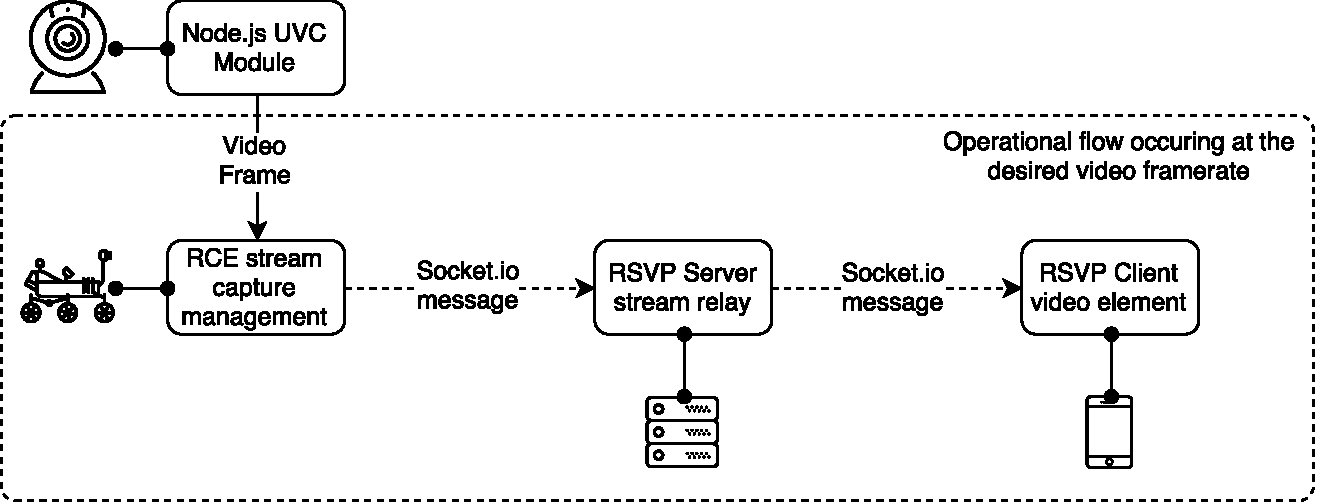
\includegraphics[width=0.8\linewidth]{figures/softDesign-socketVideoStreaming}
        \caption[Diagram of the typical flow of data using Socket.io to stream a video feed]{Diagram of the typical flow of data using Socket.io to stream a video feed}
        \label{fig:softDesign-socketVideoStreaming}
      \end{figure}
      
      Further research revealed a second streaming candidate, WebRTC, a technical specification and an open-source project comprising of APIs that can be used to implement Real Time Communications (RTC) on mobile devices and in the browser. Web-based services such as Skype, Discord, Google Hangouts and more use WebRTC for the multimedia streaming components of the applications since it provides a range of features designed a developed towards ensuring a stable communication experience despite an intermittent and unreliable network connection. An important aspect of WebRTC was the fact that the API is a part of the HTML5 specification meaning cross-browser support is driven by competition of compatibility among browser vendors, a valuable dynamic for accessibility for the project. Having said that, WebRTC have provided yet another module, \mintinline{js}{webrtc-adapter}\footnote{\mintinline{js}{webrtc-adapter} - \url{https://github.com/webrtc/adapter/}} to ensure compatibility of applications in the context of a highly volatile platform environment.
      
      In the case of the WebSocket connection technique, it is apparent that there is little to no dynamically optimised transmission of video data at any point in the transport layer meaning the video feed would have been susceptible to poor network performance resulting in severe latency and potential memory issues due to bottlenecks at the sending nodes (RCE and RSVP Server). The desired robustness would have to be developed around the use of Socket.io, a task requiring extra research and development. On the other hand, the WebRTC communications architecture, which can be seen in Figure~\ref{fig:softDesign-webRTCArch}, included a video engine as part of a rich audio-visual enhancement layer which aimed to, among other objectives, protect the stream from transmission issues. As such, WebRTC was chosen as the streaming technique and the benefits that it provided to the project will become apparent in the description below and further in the design sections.
      
      \begin{figure}[h!]
        \centering
        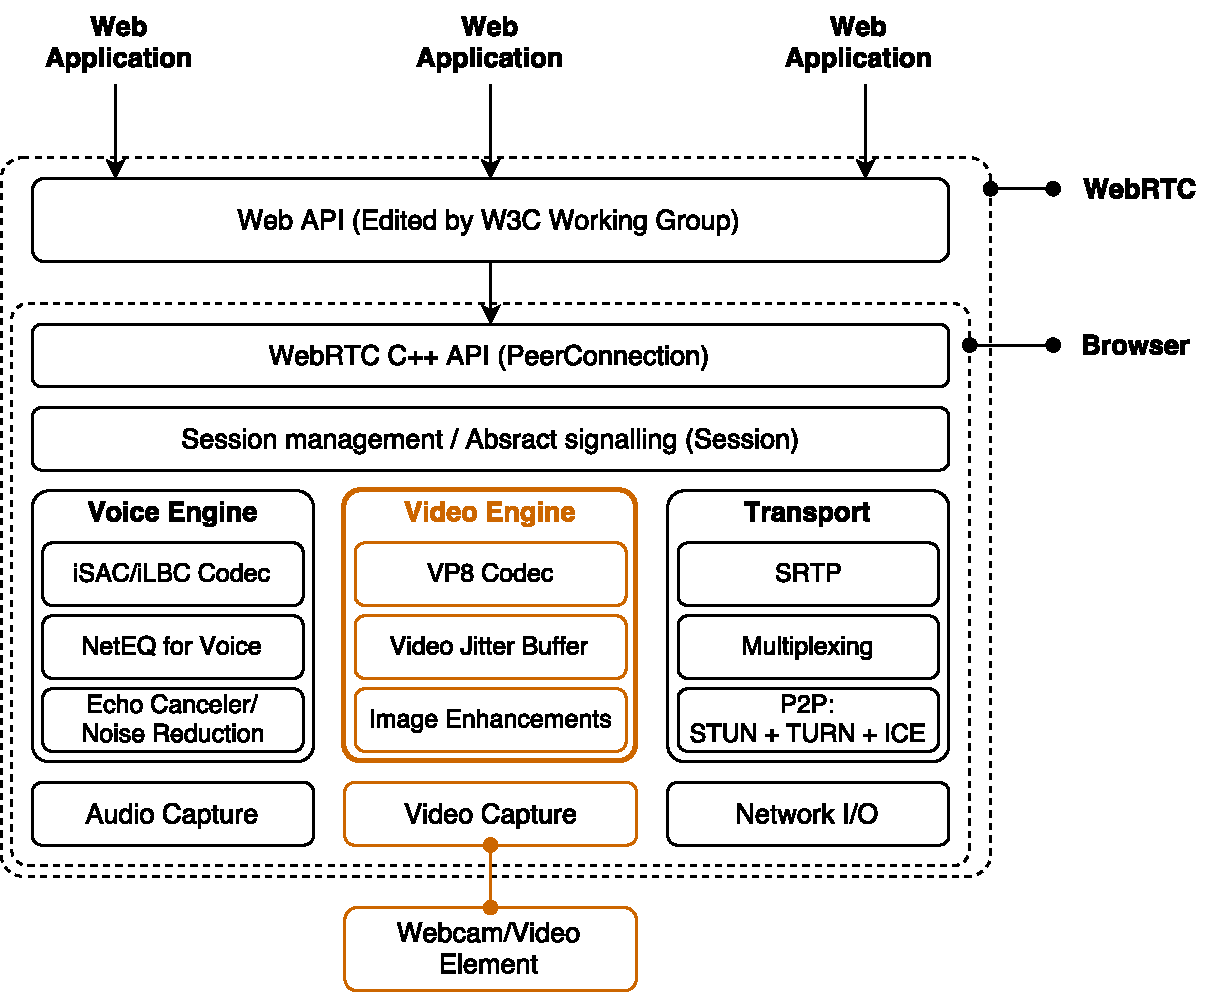
\includegraphics[width=0.8\linewidth]{figures/softDesign-webRTCArch}
        \caption[Diagram of the WebRTC architecture highlighting the video component of the streaming WebRTC provides]{Diagram of the WebRTC architecture highlighting the video component of the streaming WebRTC provides (adapted from \cite{fig:softDesign-webRTCArch_cite})}
        \label{fig:softDesign-webRTCArch}
      \end{figure}
      
      As shown in Figure~\ref{fig:softDesign-webRTCArch}, WebRTC caters for both video and audio streaming, however, only the video capabilities apply to this project. In fact, WebRTC provides arbitrary data streaming by means of an \mintinline{js}{RTCDataChannel} as well and this feature was considered for the control and telemetry message data transmission. The choice remained with WebSockets due to the simplicity of the Socket.io API and the benefits that it brought considering its suitability for the associated data type and structure. The principle of operation behind WebRTC is primarily defined by the notion of the manifestation of a session between two peers by means of the \mintinline{js}{RTCPeerConnection} component. The session can be referred to as a call, and the call handshake process involves the two peers that intend to connect and a third element, a signalling server, which facilitates the initial inter-peer communication before the session is live. A complete description of the implementation of WebRTC is given in Section~\ref{sec:softwareDevelopment}. The important point here, however, is the fact that the session is peer-to-peer, meaning video streaming from the rover to the RSVP Client need not involve an intermediate server component at all, apart from the signalling required at session initiation. Whilst this was appealing from the perspective of a simpler network configuration as well as a simpler server design, the project required one-to-many communication since the video streaming was a broadcast as opposed to a two-endpoint call. Having the $N$ number of connected RSVP Clients imposing the responsibility of broadcasting the video onto the RCE would not have been suitable given the resource and computational limitations of the Intel Edison. A preferred configuration was to have the RCE transmit the video data to the RSVP Server and have the Server be responsible for the broadcast of the data. The two configurations are contrasted in Figure~\ref{fig:softDesign-webRTCBroadcastExamples}.
      
      \begin{figure}[h!]
      \centering
      \subfloat[Without intermediate server for video streaming (strictly peer-to-peer)]{
        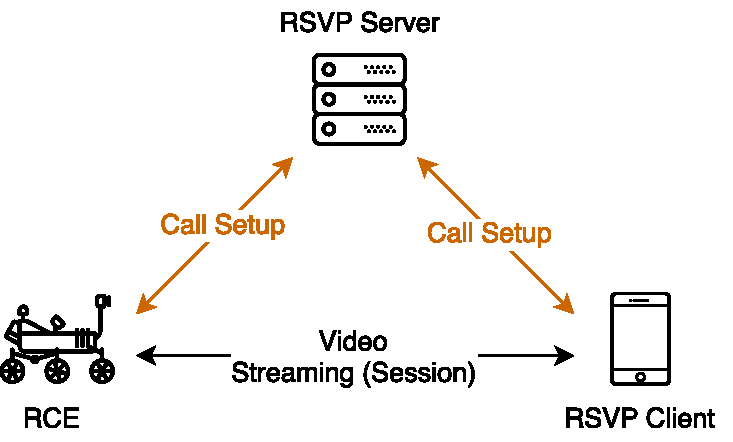
\includegraphics[width=0.49\linewidth]{figures/softDesign-webRTCBroadcastP2PExample.pdf}
      }%
      \subfloat[With intermediate server for video streaming]{
        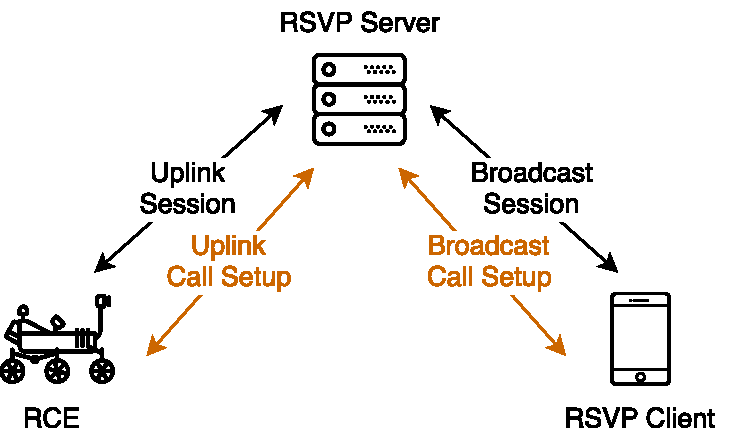
\includegraphics[width=0.49\linewidth]{figures/softDesign-webRTCBroadcastServerExample.pdf}
      }
      \caption[Simplified diagrams of typical WebRTC connection configurations]{Simplified diagrams of typical WebRTC connection configurations}
      \label{fig:softDesign-webRTCBroadcastExamples}
      \end{figure}
      
      As with the Socket.io abstraction for WebSockets, multiple services and modules were available for the implementation of a WebRTC communication system, all of which were free and consumed much of the work that would have been required for development consisting primarily of boilerplate software. The projects/modules considered included EasyRTC\footnote{EasyRTC: A comprehensive JavaScript library consisting of client and server APIs developed for multiple browsers, Node.js and signalling via Socket.io - \url{https://github.com/priologic/easyrtc}}, SimpleWebRTC\footnote{SimpleWebRTC: A simplified abstraction of the core WebRTC components and features - \url{https://github.com/andyet/SimpleWebRTC}}, Kurento\footnote{Kurento: A WebRTC media server and client APIs offering full media broadcast in multiple configurations - \url{http://www.kurento.org/}} and PeerJS\footnote{PeerJS: A browser-based WebRTC wrapper providing configurable peer-to-peer connections for arbitrary data transfer - \url{http://peerjs.com/}}. PeerJS was not suitable for the streaming-type communication required for the project and SimpleWebRTC and EasyRTC did not provide the richer media server capabilities that Kurento offered. Therefore, Kurento was chosen for the media server it included as well as the fact that it provided server-side APIs developed for Node.js together with client APIs. The Kurento media server was designed to be a common node in a broadcast network and thus suited well the use case of the project.
      
      Detailed design of the system with the implementation of Kurento's media server will be covered in the design and development sections to follow.
  \subsection{Subsystem Design}
    \subsubsection{RCE Design}
      
    \subsubsection{RSVP Server Design}
    \label{subsubsec:rsvpServersPlan}
    \subsubsection{RSVP Client Design}
    
